\section{The Unified Benchmark}

This section places all three algorithm families on one harness and
establishes the paper's organizing thesis. We report competitive ratios
(mean \(\pm\) 95\% CI) as a function of prediction quality, in three
panels chosen to span the regimes each family was designed for.

\subsection{Design}

The families consume different prediction objects, so each is driven by
its own corruption knob and reported in a parallel panel (Section 2.3);
the shared harness --- graphs, \(\mathrm{OPT}\), CI methodology, and the
advice-free floor --- is what makes the panels comparable.

\textbf{Instance format and notation.} Every panel uses the instance
format of Section 2.1: \(n\) offline resources, \(r\) online request
types, and \(m\) arrivals drawn i.i.d. from the type distribution;
throughout this section \(m=n\), so requests and resources are balanced.
The panels differ \emph{only} in the type graph connecting requests to
resources --- that single change is what moves the input between the
regimes the two prediction families were designed for. The three are
chosen so that a \emph{degree} predictor has strong signal, weak signal,
and no role at all, respectively:

\begin{itemize}
\tightlist
\item
  \textbf{Panel A --- heavy-tailed degrees (Zipf)} (\(n=1000\), 60
  trials): resource degrees follow a Zipf power law with exponent
  \(1.0\) --- a few resources are heavily contended while most are
  rarely eligible. This heavy-tailed profile gives a \emph{degree}
  predictor genuine signal to carry.
\item
  \textbf{Panel B --- left-regular \(d{=}5\)} (\(n=1000\), 60 trials):
  each arriving request connects to exactly \(d=5\) uniformly random
  resources, so resource degrees are nearly homogeneous --- the hard
  case for this family, where a degree predictor has almost no signal
  left to carry.
\item
  \textbf{Panel C --- few-types \(r{=}8\)} (\(n=2000\), 50 trials): only
  \(r=8\) distinct request types, each arriving \(\approx n/r=250\)
  times on average --- the near-perfect-matchable, few-types regime the
  \emph{histogram}-advice algorithms are calibrated for; their
  test-and-fallback test inspects a prefix of \(k=200\) arrivals.
\end{itemize}

Panels A and B thus exercise the degree-prediction family (MPD and its
augmentations); Panel C exercises the histogram-advice family
(FollowPrediction, TestAndMatch, and the combiner).

\textbf{Shared methodology.} Paired trials, independent random streams
and confidence intervals are exactly as in Section 2.5; the
panel-specific parameters are the ones listed above, and the intervals
are tight throughout (\(\pm0.001\)--\(0.003\)). The quality columns
instantiate the error models of Section 2.3 --- degree panels:
\emph{perfect} (true realized degrees), \emph{noisy} (random-flip at
strength \(\tfrac12\)), \emph{adversarial} (order-reversing reflection),
\emph{garbage} (independent random \(\mu\), \(\equiv\) Ranking); advice
panel: the true histogram blended toward a concentrated random target by
\(\eta\in\{0,0.3,0.6,1.0\}\) (\emph{perfect / mild / bad / garbage}).
The two sets of columns are \emph{not} commensurable --- they corrupt
different prediction objects with different knobs --- so only
within-panel comparisons carry meaning. \textbf{Table 1} presents each
panel's ratios beside its bar chart; the findings follow in Section 3.2.

\begin{table}[H]
\caption{The unified benchmark. Each panel's competitive ratios (means over paired
trials; every 95\% CI $\le 0.003$) sit beside their bar chart (error bars: 95\% CIs;
dashed line: advice-free floor; dotted: oracle ceiling). Bold marks the worst column of
each unguarded prediction-follower; all three fall below their own panel's floor. That
floor is instance-dependent --- it is Ranking's ratio on that panel's graph family, not a
constant --- so the three floors ($0.948$, $0.890$, $0.990$) are not comparable with one
another, and neither are the quality columns across the two prediction families
(Section 2.3).}
\footnotesize
\setlength{\tabcolsep}{4pt}
\noindent
\begin{minipage}[c]{0.62\linewidth}
\begin{tabular}{@{}lrrrr@{}}
\toprule
\emph{Panel A --- heavy-tailed (Zipf)} & perfect & noisy & advers. & garbage \\
\midrule
Ranking (floor) & 0.948 & --- & --- & --- \\
MinDegree (oracle) & 0.996 & --- & --- & --- \\
MPD & 0.989 & 0.956 & \textbf{0.908} & 0.946 \\
Feldman(MPD) & 0.981 & 0.979 & 0.976 & 0.978 \\
JailletLu(MPD) & 0.977 & 0.976 & 0.974 & 0.975 \\
Feldman (base) & 0.887 & --- & --- & --- \\
JailletLu (base) & 0.900 & --- & --- & --- \\
\bottomrule
\end{tabular}
\end{minipage}\hfill
\begin{minipage}[c]{0.36\linewidth}
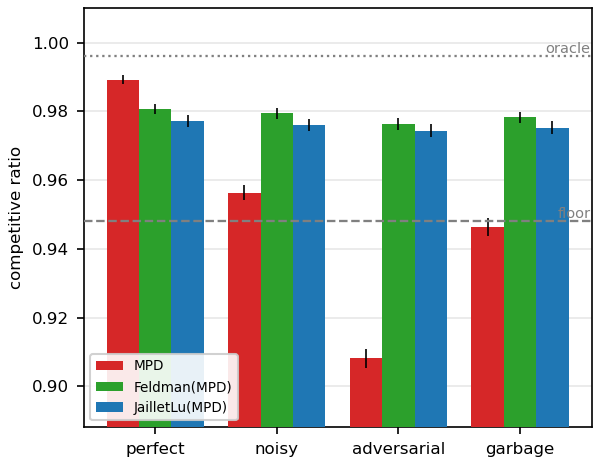
\includegraphics[width=\linewidth]{figs/unified_benchmark_panelA.png}
\end{minipage}

\medskip
\noindent
\begin{minipage}[c]{0.62\linewidth}
\begin{tabular}{@{}lrrrr@{}}
\toprule
\emph{Panel B --- left-regular $d{=}5$} & perfect & noisy & advers. & garbage \\
\midrule
Greedy $=$ Ranking (floor) & 0.890 & --- & --- & --- \\
MinDegree (oracle) & 0.966 & --- & --- & --- \\
MPD & 0.932 & 0.906 & \textbf{0.854} & 0.888 \\
Feldman(MPD) & 0.906 & 0.902 & 0.896 & 0.900 \\
JailletLu(MPD) & 0.904 & 0.903 & 0.899 & 0.901 \\
Feldman (base) & 0.760 & --- & --- & --- \\
JailletLu (base) & 0.788 & --- & --- & --- \\
\bottomrule
\end{tabular}
\end{minipage}\hfill
\begin{minipage}[c]{0.36\linewidth}
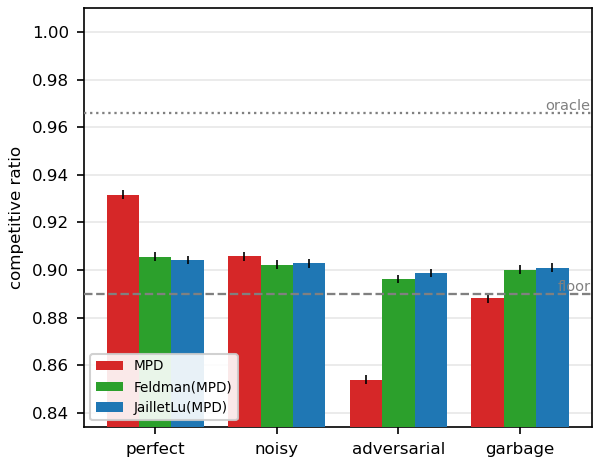
\includegraphics[width=\linewidth]{figs/unified_benchmark_panelB.png}
\end{minipage}

\medskip
\noindent
\begin{minipage}[c]{0.62\linewidth}
\begin{tabular}{@{}lrrrr@{}}
\toprule
\emph{Panel C --- few-types $r{=}8$} & perfect & mild & bad & garbage \\
\midrule
Ranking (floor) & 0.990 & --- & --- & --- \\
MinDegree (oracle) & 0.999 & --- & --- & --- \\
FollowPrediction & 1.000 & 0.832 & 0.679 & \textbf{0.472} \\
TestAndMatch (Choo) & 1.000 & 0.984 & 0.989 & 0.990 \\
TestAndMatch (BEM) & 0.998 & 0.988 & 0.988 & 0.968 \\
Combiner \emph{(benchmark)} & 0.990 & 0.990 & 0.990 & 0.990 \\
\bottomrule
\end{tabular}
\end{minipage}\hfill
\begin{minipage}[c]{0.36\linewidth}
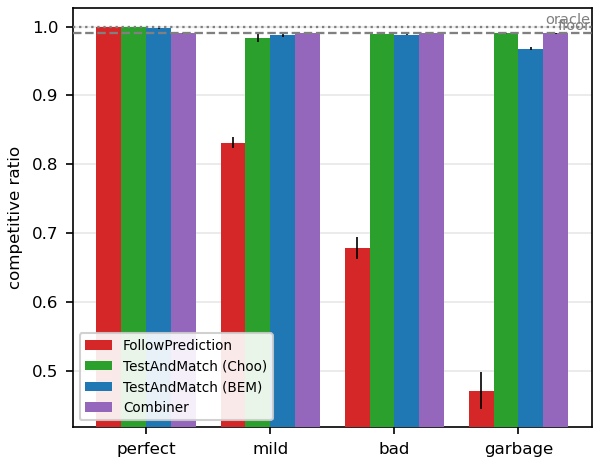
\includegraphics[width=\linewidth]{figs/unified_benchmark_panelC.png}
\end{minipage}
\end{table}

\subsection{Four findings}

\textbf{(F1) Robustness is engineered, not free: naive followers crash
below the floor.} Both unguarded prediction-followers dive under the
advice-free Ranking floor once the prediction is adversarial or garbage:
MPD falls to \(0.908 < 0.948\) (Panel A, adversarial) and
\(0.854 < 0.890\) (Panel B), and FollowPrediction collapses to
\(0.472 \ll 0.990\) (Panel C). Under adversarial or garbage advice,
then, a practitioner using either \emph{unguarded} is worse off than
using no prediction at all --- at perfect and noisy advice the same
algorithms sit above the floor. Every \emph{robust} algorithm in the
tables --- the augmentations, TestAndMatch, the combiner --- avoids this
by construction, not by luck.

\textbf{(F2) Two distinct robustness mechanisms, with different shapes.}
\emph{Structural} robustness (Feldman(MPD), JailletLu(MPD)): a
worst-case-optimal base matching carries the load and the prediction
only breaks ties, so performance is nearly \emph{flat} across quality
--- Feldman(MPD) moves only \(0.981\!\to\!0.976\) from perfect to
adversarial (Panel A). It cannot crash, but it also caps the upside (it
never reaches the \(0.996\) oracle, and sits below MPD's \(0.989\) at
perfect). \emph{Adaptive} robustness (TestAndMatch): test a sublinear
prefix, then commit --- capturing the upside when advice is good (Choo
\(1.000\) at perfect) \emph{and} holding the floor when advice is bad
(\(0.990\) at garbage). On Panel C it is the only algorithm on the upper
envelope at both ends. The two mechanisms trade consistency for
robustness in opposite ways.

\textbf{(F3) The consistency upside is small on average-case inputs; the
spread lives on the bad-advice side.} On few-types the advice-free
Ranking is already \(0.990\) and MPD-with-true-degrees is \(0.999\) ---
under \(0.01\) for \emph{any} advice to add on the good side. Every wide
gap in Panel C (\(1.000\!\to\!0.472\) for FollowPrediction; the
half-wide envelope) is a \emph{downside} gap. This is the thesis in one
panel: learning-augmented matching on typical inputs is robustness
insurance, not a performance lift --- a fact Section 7 prices: safely
capturing an upside this small would take a longer prefix than the
instance itself.

\textbf{(F4) The augmentation rescues structurally weak base
algorithms.} Feldman and Jaillet--Lu are tuned for the worst-case ratio
and are the \emph{weakest} advice-free entries on these average-case
inputs (Panel B: \(0.760\) / \(0.788\), well below Greedy's \(0.890\)).
The MPD augmentation lifts them to \(\approx 0.90\) --- the prediction
does \emph{more} for the worst-case-designed algorithms than for greedy.
This pairing is visible only under a unified table.

\subsection{Takeaway}

Read together, F1--F4 say that on average-case matching the advice-free
baseline is already near-optimal, unguarded prediction-following is
unsafe, and the value of the sophisticated algorithms is downside
protection delivered by one of two mechanisms. Sections 4--6 sharpen and
stress-test each part --- what governs the (small) loss, what the
adaptive test costs, and whether the picture survives on real graphs,
real traces, and a learned predictor --- and Section 7 proves the wall
is not an artifact but a price: a budget--stakes law that puts the
required test prefix beyond the horizon exactly where the baseline is
strong.
